\chapter{Structural and accidental gaps} \label{clusters}

Early work in generative phonology recognized that neutralizing, surface-true phonological alternations constrain possible surface forms and possibly, lexical entries (\citealp[283]{Anderson1974}, \citealp[382]{SPE}, \citealp[205f.]{Dell1973}, \citealp[22f.]{SPR}, \citealp{Kenstowicz1977}: chapter 3, \citealp[28f.]{Stampe1979}, \citealp[410f.]{Stanley1967}). Despite isolated claims to the contrary (e.g., \citealp[297]{Hale1965}; \citealp[212f.]{Postal1968}), however, the curent \emph{communis opinio} holds that speakers' knowledge of phonotactics---that is, language-specific sound sequence co-occurrence restrictions---is partially independent of the phonology proper. 

\begin{quote}
It would be a result of the greatest interest if it were to turn out that every intramorphemic regularity was necessarily reflected in an alternation, and thus in a rule; but this position cannot seriously be maintained. \citep[283]{Anderson1974}
\end{quote}

This chapter argues that the only structural constraints on possible syllable contact clusters in English are derived from phonological alternations. This result serves to undermine the hypothesis of an independent phonotactics module, insofar as this particular domain has been used, by \citet{Pierrehumbert1994} and others, to illustrate the necessity of such a module and to outline proposals for its architecture.  

\section{Background}

\subsection{Phonotactics and the morph}

Linguists have long recognized the morph as a privileged domain for phonotactic generalizations. 

A major result of American structuralism is that generalizations which hold of the sound sequences found in underlying forms may not hold across morph boundaries. In his history of phonology, \citet[][267]{Anderson1985} indirectly credits this insight to \citet{Bloomfield1930}, who proposes that a problem in the phonemic analysis of German can be resolved by allowing for allophony to make reference to morpheme boundaries. \citeauthor{Bloomfield1930} notes that [ç] and [x] can be cast as allophones, despite the existence of apparent minimal pairs like \emph{Kuchen} [kuːxən] `cake' $\sim$ \emph{Kuhchen} [kuːçən] `cow-let'. \citeauthor{Bloomfield1930}'s claim is that these words differ not just in their medial consonsant but also that the latter is a compound, marked with the diminutive \emph{-chen} (cf. \emph{Kuh} `cow'). Under the standard analysis that [x] is the allophone of /ç/ before back vowels, all that needs to be added is a restriction that the conditioning vowel belongs to the same word (or perhaps morph). 

A more sophisticated approach to problems of this type, making no reference to \citeauthor{Bloomfield1930}, was published only two years later. \citet{Jakobson1932}, then a member of the Prague circle, attributes a number of phonological properties of the Russian imperative to morph juncture. Nearly all Russian infinitives are marked with a final theme vowel and /-t\pal{}/; in reflexives, this is followed by a suffix realized as [s\pal{}ə], which triggers a general process of regressive voicing assimilation. In the reflexive infinitive, the palatalization of infinitive /-t\pal/ is lost, but in the reflexive imperative, palatalization of a stem-final consonant is preserved, even when the root-final consonant is /t\pal/, as in (\ref{rusreflex}c).\footnote{Thanks to Lev Blumenfeld for assistance with this data.}

\begin{example}[Russian reflexives] \label{rusreflex}
\begin{tabular}{l l l l}
   &  infinitive       & imperative \\
a. & [slav\pal{}itsə]  & [slaf\pal{}s\pal{}ə]  & `be glorious'   \\
   & [upram\pal{}itsə] & [upram\pal{}s\pal{}ə] & `be stubborn'   \\
b. & [kras\pal{}itsə]  & [kras\pal{}s\pal{}ə]  & `put on makeup' \\
   & [ʒar\pal{}itsə]   & [ʒar\pal{}{}s\pal{}ə] & `roast'         \\
c. & [zəbytsə]         & [zəbut\pal{}s\pal{}ə] & `forget'        \\
\end{tabular}
\end{example}

\noindent \citeauthor{Jakobson1932} proposes that the preservation of palatalization in /\ldots{}t\pal{}-s\ldots{}/ is a special property of the imperative. Both (\ref{rusreflex}c) forms contain a /t\pal-s/ juncture, though palatalization is only preserved in the imperative. \citeauthor{Jakobson1932} proposes that the phonology treats them differently: the imperative does not undergo loss of palatalization. A few years later, \citet{Trnka1936} makes the connection between \citeauthor{Jakobson1932}'s hypothesis and phonotactic generalizations. 

This is apparent from a discussion of constraints on vowel sequences in Mixteco (a dialect cluster also known as Mixtec) given by \citet{Pike1947b}. It is apparent that \citeauthor{Pike1947b}'s constraints on vowel sequences are not intended to hold across morph boundaries, according to the phonological analysis of a Mixteco text published a few years earlier \citep{Pike1944}. A few examples are given below; the transcriptions are \citeauthor{Pike1944,Pike1947b}'s.

\begin{example}[Mixteco MSCs and complex words \citep{Pike1944,Pike1947b}]
\begin{tabular}{l l@{} l l l}
a. & * & {C}a{C}e & [ká\textsuperscript{n}dee]    & `kept inside'   \\
b. & * & {C}ə{C}e & [nìk\`əbəde]                  & `who entered'   \\
c. & * & {C}e{C}i & [teníke\textsuperscript{n}da] & `was walking    \\
d. & * & {C}i{C}e & [tenìkeet\`ə]                 & `and went away' \\
\end{tabular}
\end{example}

\noindent \citet[][166]{Pike1947b} affirms that the morpheme is ``marked'' by the violation of morpheme-internal sequence restrictions, an idea further developed by \citet{Harris1955} as a discovery procedure for morphs (see also \citet{Hafer1974}).

\subsubsection{Early generativism}

\citet{SPR,Halle1962} and \citet{Chomsky1965,SPE} posit a system of a system of \emph{morpheme structure constraints}---more precisely, \emph{sequence structure constraints} \citep{Stanley1967}---used to fill out redundant specifications in underlying forms, and to account for speakers' knowledge of possible words.

\subsubsection{Gradient patterns}


\section{Evaluation}

This study 

% The subject of this study are medial clusters

\subsection{Data sources}

A list of medial clusters is gathered by applying a number of filters and transformations to an English lexical database. The resulting list of clusters is reproduced in Appendix \ref{appendixB} and in electronic form at the author's website.

\subsubsection{Identifying simplex words}

An analysis of lexical constraints requires a corpus of lexical representations. So as to remain agnostic about particulars of morphological theory, the goal here is to identify words which bear no overt inflection, and which do not admit any plausible further decomposition, henceforth ``simplex words''. For the structuralists, a procedure for parsing words into morphs, just the thing for locating simplex words, held the status of ``philosopher's stone'', a sort of near-mythical objective of the endeavour, but actual attempts to develop such a procedure \citep[e.g.,][]{Harris1955,Nida1948} are now recognized as anything but theory-neutral. Yet, there is no alternative to adopting some computational procedure or human-coded database as the ``gold standard'' for a study of this type. \citet{Pierrehumbert1994} analyzes a list of entries in the Collins English dictionary by hand, using her intuitions to filter out ``complex'' words as well as those which are not ``reasonably familiar''. Unfortunately, the resulting list was neither published nor circulated, and the possibility of replicating \citeauthor{Pierrehumbert1994}'s' sensations of morphological complexity is remote. Following prior studies of syllable contact clusters by \citet[ chapter 3]{Hammond1999a} and \citet[ chapter 8]{Duanmu2009}, a list of simplex words was derived from the ``lemmas'' (that is, uninflected forms) in the English portion of CELEX \citep{CELEX}, a database of morphological, phonological, and syntactic annotations based on the COBUILD corpus, a resource that was also used to construct the Collins English dictionary employed by \citeauthor{Pierrehumbert1994}.

Two further filters were applied to this list. First, any lemma coded as an unassimilated loanword is excluded. Secondly, all lemmas that have a ``morphological status'' other than ``monomorpheme'' are excluded. This is crucial because CELEX makes no guarantee that lemmas are simplex; indeed, many lemmas are products of derivation (e.g., \emph{abusive}, from \emph{abuse}). These stringent criteria have a profound effect on the makeup of the data. For instance, nearly all exceptions to \textsc{Obstruent Voice Assimilation} (see \S\ref{ova} below) cited by \citet[74]{Hammond1999a} are excluded as unassimilated loanwords (e.g., \emph{vodka}, \emph{smorgasbord}) or as morphologically complex (e.g., \emph{jurisdiction}, \emph{madcap}, \emph{tadpole}, \emph{scapegoat}, \emph{magpie}). 

One problematic case are the ``neo-classical compounds'', words that appear to consist of a Latinate prefix and a bound stem, like \emph{inspect} or \emph{excrete}. 


%However, it is troublesome to use these principles to argue for an otherwise-unmotivated morph juncture if the argument is only being made to preserve the very phonotactic generalization used to motivate the juncture in the first place. Unfortunately, this is the structure of \citeauthor{Pierrehumbert1994}'s discussion of \emph{antler}: her theory rules out coda coronal obstruents (like /t/) in trisyllabic clusters, and complex medial codas like /nt/ \citep[though cf.][]{Borowsky1989}, and therefore she assumes that \emph{antler} is polymorphemic and thus /nt.l/ is unattested in simplex words. Repeated indefinitely, this sort of argument would produce morphological analyses that were little more than syllabifications.

In this vein, \citet[11--13]{Aronoff1976} observes that Latinate forms which share the same bound stem also share irregular allomorphs of that stem under derivation, which he takes as evidence for prefix/bound stem decomposition. Similar behaviors are found in Russian verbs which share roots but which take different prefixes or the reflexive \citep{Pesetsky1977}.

\begin{example}[Bound stem-specific allomorphy]
\begin{tabular}{l l l}
a. & \emph{adhere}   & \emph{adhesion}   \\
   & \emph{cohere}   & \emph{cohesion}   \\
b. & \emph{conceive} & \emph{conception} \\
   & \emph{perceive} & \emph{perception} \\
\end{tabular}
\end{example}

There is also a syntactic interaction between Latinate prefixes on verbs and the makeup of the verbal complement. \citet{Harley2009} observes that Latinate verbs do not generally participate in ditransitive, verb participle, or adjectival resultative constructions, all acceptable with similar Anglo-Saxon verbs \citep[see also][]{Gropen1989,Coppock2008}. \citeauthor{Harley2009} proposes that the Latinate prefix is introduced in a low small clause, the same position as the theme, participle, and result adjectival in the Anglo-Saxon examples.

\begin{example}[Latinate verbs and small clauses] \label{harley}
\begin{tabular}{ll@{}ll@{}l}
a. & * & \emph{exhibit him the painting} & ~ & \emph{show him the painting} \\
b. & * & \emph{imbibe himself stupid}    & ~ & \emph{drink himself stupid}  \\
c. & * & \emph{exhibit it off}           & ~ & \emph{show it off}           \\
\end{tabular}
\end{example}

Furthermore the decomposition of neo-classical compounds is observed in a number of lexical decision experiments. In general, it is known that simplex words are recognized faster than complex words \citep{Caramazza1988}. Among nonce words, those that can be exhaustively decomposed into prefix and bound stem (like *\emph{de-juvenate}) are recognized slower that contain a licit morph but cannot be exhaustively decomposed (like *\emph{de-pertoire}), and these in turn are recognized slower than those which admit no such decomposition \citep{Taft1975}.\footnote{The same contrasts are present in many other domains where decomposition into root and affix(es) is far less controversial, for instance, inflected verbs in Italian \citep{Caramazza1988,Chialant1995}.} \citet{Emmorey1989} reports facilitative auditory priming between \emph{permit} and \emph{submit} \citep[though cf.][]{Marslen-Wilson1994}, and \citet{Taft2004a} find facilitative masked priming between orthographically presented pairs like \emph{virus}--\emph{viral}, but not \emph{future}--\emph{futile}, which do not share a possible bound stem.\footnote{Many have argued that full decomposition is only one of the two methods for the processing of complex words, the other being whole word looking, either running in serial \citep{Caramazza1988} or in parallel \citep{Baayen1997b}. Whatever evidence that is amassed in support of a whole word lookup procedure, however, does not undermine the considerable evidence for decomposition.}

\subsubsection{Syllabification and phonologization}

CELEX provides broad transcriptions of individual wordforms which also include syllable boundaries. However, the syllabification procedure used is not described in the documentation, and an inspection of the data reveals various unsystematic elements. In a list of English simplex words, for instance, a medial cluster and adjacent nuclei should always be syllabified in the same fashion, since there is no convincing evidence for truly ``contrastive'' syllabification in any language \citep[see]{Elfner2006}. But many syllabification contrasts can be found in the CELEX data, for instance between \emph{chemistry} [ˈkɛ.mɪ.strɪ] and \emph{ministry} [ˈmɪ.nɪs.trɪ].\footnote{Note that word-final \emph{y} is generally lax [ɪ] in Received Pronunciation \citep[][II.294]{AOE}.} This putative [ɪ.strɪ $\sim$ ɪs.trɪ] contrast does not conform to any native speaker intuition.

For this reason, an automated syllabification procedure was developed to separate medial clusters in the CELEX  monomorphs into coda and onset. Since this procedure is applied only to medial clusters, it is possible to remain agnostic on several contentious issues concerning syllabification of English; for instance, there is no need to address the status of so-called ``ambisyllabic'' consonants, since this does not occur with medial clusters, or morphological effects on syllabification, since only monomorphs are used. 

The technique used is a variation on the theme of onset maximization (e.g., \citealt{Kurylowicz1948}, \citealt[75]{Pulgram1970}, \citealt[42f.]{Kahn1976}, \citealt[][358f.]{Selkirk1982b}) which favors parses of word-medial clusters in which as much of the cluster as possible is assigned to the onset. Just what is a ``possible'' medial onset is defined by the onsets that occur in initial position \citep[though cf.][36]{Fischer-Jorgensen1952}. Medial clusters in words like \emph{neu}[.tr]\emph{on} or \emph{bi}[.str]\emph{o} are found in word-initial position (e.g., [tr]\emph{ansit}, [str]\emph{ike}), so onset maximization assigns the entire medial cluster to the onset, leaving the medial coda empty. In contrast, the [nstr] cluster in \emph{mi}[n.str]\emph{el} is not found word-initially; the maximal onset here is [str], and the residual [n] is assigned to the coda.

There is one case where unchecked maximization of medial onsets produces incorrect syllabifications. When a medial consonant cluster is preceded by a stressed lax vowel, as in words like \emph{wh}[ɪs.p]\emph{er}, \emph{v}[ɛs.t]\emph{ige}, or \emph{m}[ʌs.k]\emph{et}, the first consonant of the cluster checks the lax vowel \citep[e.g.,][3]{Hammond1997}. \citet[][55]{Harris1994} notes that onset maximization produces an incorrect result when a stressed lax vowel is followed by a medial cluster which is also a valid onset: in \emph{whisper}, \emph{vestige}, and \emph{musket}, it incorrectly assigns [sp, st, sk] to the medial onset, leaving the coda empty. The approach adopted here is is to assign the first consonant of a medial cluster to the coda of a preceding syllable if it follows a stressed lax vowel \citep[cf.][48]{Pulgram1970}.

The previous principle has the potential to introduce a related issue for parsing medial affricates. Since the \emph{Grundzüge der Phonologie} \citep{Trubetzkoy1958}, first published in 1939, affricates are understood as single plosive segments distinguished from pure stops by the presence of stridency \citep[24]{Jakobson1961} or a delayed release (\emph{SPE}:321f). If however, the English affricates [tʃ, dʒ] are treated as stop-fricative sequences \citep[e.g.,][]{Hualde1988,Lombardi1990}, this procedure will incorrectly assign the two components of the medial affricate to separate syllables before stressed lax vowels (e.g., \emph{ra}[.tʃ]\emph{et} or \emph{a}[.dʒ]\emph{ile}) unless there is an ad-hoc constraint that treats these sequences as indivisible \citep[e.g.,][]{Wells1990}. Here, the traditional treatment of affricates as single segments is assumed. This assumption can be motivated by the tendency of affricates to pattern with individual segments in phonotactic generalizations. For instance, Classical Nahua allows the affricate series [ts, tʃ, tɬ] in onsets, but bans all other onset clusters \citep[9]{Launey2011}.%, and \citet[86]{Butskhrikidze2002} notes a similar generalization in the consonant clusters of Geor

This potentially introduces a problem with medial affricates. At least as far back as the 1939 first edition of the \emph{Grundzüge der Phonologie} \citep{Trubetzkoy1958}, affricates have been analyzed as single plosive segments distinguished from stops by the presence of stridency \citep[24]{Jakobson1961} or a delayed release (\emph{SPE}:321f). If however, the English affricates [tʃ, dʒ] are treated as stop-fricative sequences (e.g., \citealt{Hualde1988}, \citealt{Lombardi1990}), this procedure will incorrectly assign the two components of the medial affricate to separate syllables before stressed lax vowels (e.g., \emph{ra}[.tʃ]\emph{et} or \emph{a}[.dʒ]\emph{ile}) unless there is an ad-hoc constraint that treats these sequences as indivisible \citep[e.g.,][]{Wells1990}. Here, the traditional treatment of affricates as single segments is assumed. This assumption can be motivated by the tendency of affriates to pattern with individual segments in phonotactic generalizations. For instance, Classical Nahua allows the affricate series [ts, tʃ, tɬ] in onsets, but otherwise does not permit other onset clusters \citep[9]{Launey2011}, and \citet[86]{Butskhrikidze2002} notes a similar generalization in the consonant clusters of Georgian.

\subsubsection{Subsyllabic parsing}

It is also necessary to separate the interlude from the nuclei on either side. Distributional heuristics are used to develop a subsyllabic parsing procedure for English below.

\paragraph{The velar nasal} There is a long-standing debate regarding whether English [ŋ] is a phoneme in its own right \citep[e.g.,][]{Sapir1925}, an analysis which is a consequence of principles like the Alternation Condition \citep{Kiparsky1968} or Lexicon Optimization \citep[53]{OT}, or simply the allophone of /n/ when followed by underlying /k, ɡ/ (e.g., \emph{SPE}:85, \citealt{Borowsky1986}:65f.), sometimes followed by the deletion of /ɡ/. The strongest piece of evidence for the latter position, in which the velar nasal is a pure allophone, is the general absence of onset [ŋ], a position where it can never be followed by a dorsal consonant needed to derive the velar allophone. Following \citet{Pierrehumbert1994}, the pure allophonic analysis is adopted here, and English nasal place allophony is formalized in Section \ref{npasection} below.

\paragraph{[j] onglides} While some have assumed that the front onglide in words such as \emph{val}[j]\emph{ue} is inserted by rule (\emph{SPE}:196, \citealt[][89]{Halle1985a}, \citealt[][217]{McMahon1990}), the very presence or absence of the glide is in fact contrastive (e.g., \emph{coo}/\emph{coup} \alt{} \emph{queue}, \emph{booty} \alt{} \emph{beauty}) and thus assumed to be present in underlying representation (\citealt{Anderson1988b}, \citealt[278]{Borowsky1986}). The front onglide is further assumed to be assigned to the nucleus, except when the onset would otherwise be null (e.g., \emph{jun}[j]\emph{or}). There is considerable evidence for this assumption. When [j] is a simplex onset, it may be followed by any vowel \citep[][276]{Borowsky1986}, but when [j] is immediately preceded by an onset consonant (e.g., [bj]\emph{ugle}), the following vowel is always [uː]. This defective distribution of vowels following [j] suggests that the onglide in this context is the first component of an underlyingly complex vowel segment (\citealp[][232]{Hayes1980}, \citealp[][61f.]{Harris1994}, \citealp{Davis1995}). \citet[][42]{Clements1983} note that /m, v/ do not appear in onset clusters, though they may be followed by [ju] in words like [mj]\emph{use} or [vj]\emph{iew}, also suggesting the nuclear affiliation of the glide. There is also strong external support for this principle. The [ju] in words like \emph{spew} may pattern together in Pig Latin \citep{Davis1995,Idsardi2005}, \emph{shm}-reduplication \citep{Nevins2003}, and speech errors (e.g., [kjuː]\emph{mor} [h]\emph{omponent} for intended [hju]\emph{mor component}; \citealt[130]{Shattuck-Hufnagel1986}).

\paragraph{[w] onglides} The phonotactic properties of the back onglide [w] are the opposite of the front onglide. Whereas the front onglide shows only limited selectivity for preceding tautosyllabic consonants \citep{Davis1995,Kaye1996}, the back onglide [w] is rarely preceded by tautosyllabic consonants other than [k] (e.g., \emph{tran}[kw]\emph{il}). Unlike the front glide, syllable-initial [kw] may be followed by nearly any vowel \citep[161]{Davis1995}. Unlike [juː], onglide [w] followed by a vowel does not pattern together in Pig Latin \citep[166]{Davis1995}. Taken together, these facts indicate that the back onglide is assigned to the onset.

\paragraph{Post-vocalic \emph{r}} Both CELEX and the dictionary used by \citet{Pierrehumbert1994} transcribe Received Pronunciation, in which word-medial post-vocalic \emph{r} has been lost. Even in \emph{r}-full dialects, though, there is reason to believe that post-vocalic \emph{r} is in fact nuclear, and therefore its presence or absence is irrelevant to the constraints on syllable contact clusters. Many vowel contrasts are suspended before \emph{r} (e.g., \citealt[269f.]{Fudge1969}, \citealt[][255]{Harris1994}); for example, \emph{fern}, \emph{fir}, and \emph{fur} lack the contrasts found in \emph{pet}, \emph{pit}, and \emph{putt}. Further evidence for the nuclear status of post-vocalic \emph{r} comes from variable phonological processes in which it patterns differently than internal coda consonants. \citet[258]{Harris1994} reports that post-vocalic \emph{r} is the only consonant which does not block a variable process of /t/-\textsc{Glottalization} found in many British dialects.

\begin{example}[/t/-\textsc{Glottalization} in British English]
\begin{tabular}{l l l l@{} l}
a. & \emph{des}[ɚt]         & \alt{} &   & \emph{des}[ɚʔ]         \\
   & \emph{c}[ɚt]\emph{ain} & \alt{} &   & \emph{c}[ɚʔ]\emph{ain} \\
b. & \emph{fi}[st]          & \alt{} & * & \emph{fi}[sʔ]          \\
   & \emph{mi}[st]\emph{er} & \alt{} & * & \emph{mi}[sʔ]\emph{er} \\
\end{tabular}
\end{example}

\noindent Whereas post-vocalic \emph{r} is the only consonant which fails to block /t/-\textsc{Glottalization} in British dialects, it is the only consonant which fails to feed /t, d/-\textsc{Deletion} in American English \citep[8]{Guy1980}.

\begin{example}[/t, d/-\textsc{Deletion} in American English] \label{td}
\begin{tabular}{l l l l@{} l}
a. & \emph{be}[lt] & \alt{} &   & \emph{be}[l] \\
   & \emph{me}[nd] & \alt{} &   & \emph{me}[n] \\
b. & \emph{sh}[ɚt] & \alt{} & * & \emph{sh}[ɚ] \\
   & \emph{c}[ɚd]  & \alt{} & * & \emph{c}[ɚ]  \\
\end{tabular}
\end{example}

\subsubsection{Lexical statistics}

The English portion of CELEX contains 6,876 simplex words with 21 unique medial codas and 40 unique medial onsets. Of the 840 ($= 21 \times 40$) possible syllable contact clusters that could be produced by free combinations of the attested medials codas and onsets, 158 are attested, an 18.8\% saturation rate. The data set is reproduced in Appendix \ref{appendixB}.

\subsection{Static and derived constraints}

\emph{SPE} describes three phonological alternations which target syllable contact clusters. The corresponding constraints on simplex syllable contact clusters are considered below. The first such derived constraint, obstruent voice assimilation, is presented as a tutorial introduction. The second set of constraints consists of three static phonotactic constraints proposed by \citet{Pierrehumbert1994}.

\subsubsection{Obstruent voice assimilation} \label{ova}

Voice assimilation in English is exemplified by the allomorphs of /-d/ suffix, forming regular pasts and denominal adjectives, and the /-z/ suffix, forming regular noun plurals, genitives, and the 3sg. present active indicative.\footnote{The URs /-d, -z/ are argued for by \citet[282]{Hockett1958}, \citet[210]{SPE}, \citet{Basboll1972}, \citet{Shibatani1972}, \citet{Anderson1973a}, \citet[102]{Pinker1988}, and \citet[284f.]{Bakovic2005b}; alternatives are suggested by \citet[210f.]{LANGUAGE}, \citet[426]{Nida1948}, \citet{Luelsdorff1969}, \citet{Lightner1970}, \citet{Hoard1971}, \citet{Miner1975}, \citet{Zwicky1975}, \citet{Kiparsky1985}, and \citet[135]{Borowsky1986}.}

\begin{example}[Inflectional affix voice assimilation]
\begin{tabular}{llllll}
a. & \emph{nap} & \emph{nap}[t] \\
   & \emph{nab} & \emph{nab}[d] \\
b. & \emph{lap} & \emph{lap}[s] \\
   & \emph{lab} & \emph{lab}[z] \\
\end{tabular}
\end{example}

\noindent The devoicing of the two voiced obstruent suffixes can be formalized as a rule spreading the voicing specification of an obstruent rightward. 

\begin{example}[\textsc{Obstruent Voice Assimilation} (after \emph{SPE}:178)]
\xymatrix@R=24pt@C=24pt{
\txt{[α \textsc{Voice}]}\ar@{-}[d]\ar@{--}[dr] &                               \\
\txt{C}\ar@{-}[d]                              & \txt{C}\ar@{-}[d]             \\
\txt{[$+$\textsc{Obstruent}]}                  & \txt{[$+$\textsc{Obstruent}]} \\
}
\end{example}

It is quite apparent that root-internal hetero-voiced obstruent clusters like [s.b] or [z.t] are rare compared to clusters which are uniformly voiced or uniformly voiceless, as predicted the assimilation rule. Yet, \citet{Pierrehumbert1994} does not mention voice assimilation in her study of English syllable contact clusters. \citet[]
[74f.]{Hammond1999a} cites words like \emph{a}[b.s]\emph{inth} and \emph{a}[s.b]\emph{estos}, which contain hetero-voiced obstruent clusters, as evidence that the proce
ss does not apply to simplex words. Indeed, the \textsc{Revised Alternation Condition} (RAC) proposed by \citeauthor{Kiparsky1973a} (\citeyear{Kiparsky1973a}:163, \citeyear{Kiparsky1982a}:152) blocks the application of obligatory neutralization processes like \textsc{Obstruent Voice Assimilation} in root-internal (i.e., non-derived) environments.\footnote{The ``obligatory'' condition on the RAC has the unforunate result that \textsc{Obstruent Voice Assimilation} is always consistent with the RAC whether or not it actually applies in non-derived environments. If the rule applies in non-derived environments, then it has lexical exceptions (e.g., \emph{a}[s.b]\emph{estos}) and is not obligatory and thus free from the RAC. On the other hand, if the rule is subject to the RAC, it only applies in derived environments, in which it is obligatory.} 

The question can be stated in the form of a statistical test: does \textsc{Obstruent Voice Assimilation} (posited to apply in non-derived environments) account for a meaningful generalization about the lexicon (henceforth, the alternative hypothesis) or is it indistinguishable from noise (the null hpypothesis)? 

This question is answered by considering the subset of the 840 ``possible'' clusters in which the final coda consonant and the first onset consonant are both obstruents: there are 720 in all. These are then sorted into 4 bins, according to whether or not they are attested or not, and whether or not they conform to the generalization---that is, whether both are voiced or voiceless, like in \emph{hu}[z.b]\emph{and} or \emph{ma}[s.t]\emph{iff}, respectively---or violate it, like the aforementioned \emph{a}[b.s]\emph{inth} and \emph{a}[s.b]\emph{estos}. The resulting table is shown in (\ref{ova}) below. 18\% of the possible clusters containing adjacent obstruents agreeing in voicing are found in the corpus, whereas only 2\% of those which disagree in voicing are attested. The table is then submitted to the Fisher Exact Test. The resulting very small $p$-value indicates that the rarity of the disagreeing clusters is unlikely to be due to chance. The simplest interpretation of this fact is that \textsc{Obstruent Voice Assimilation} applies in non-derived environments, preventing learners from positing URs in which adjacent obstruents do not agree in voice.

\begin{example}[Lexical effects of \textsc{Obstruent Voice Assimilation}] \label{ova}
\begin{tabular}{l r r r r}
\toprule
           & attested & unattested & saturation & $p$-value                   \\
\midrule
conforming & 80       & 370        & 0.178      & \multirow{2}{*}{1.1\e{-11}} \\
violating  &  6       & 264        & 0.022                                    \\
\bottomrule
\end{tabular}
\end{example}

There are two possibilities for the small number of roots that violate the derived generalization. Some hetero-voiced obstruent clusters, like the one in \emph{ja}[k\#d]\emph{aw}, for instance, might be analyzed as compounds by native speakers (cf. \S\ref{slave} above). Less informatively, exceptionality can be derived from the \emph{SPE} rule exception convention, by marking exceptional roots with the feature [$-$\textsc{Obstruent Voice Assimilation}].

\subsubsection{Nasal place assimilation} \label{npasection}

In addition to the [ŋ] allophone, \textsc{Nasal Place Assimilation} is responsible for the allomorphs of the \emph{im-}/\emph{in-} prefix. In (\ref{nparule}a), the prefix-final consonant takes on the same major place of articulation as the following obstruent. The vowel-initial bases in (\ref{nparule}b) demonstrate that the prefix is underlyingly /ɪn-/.

\begin{example}[\emph{im-}/\emph{in-} allomorphy] \label{nparule}
\begin{tabular}{l l l l}
a. & \emph{balance}   & \emph{i}[m.b]\emph{alance}  \\
   & \emph{decent}    & \emph{i}[n.d]\emph{ecent}   \\
b. & \emph{elegant}   & \emph{i}[n]\emph{elegant}   \\
   & \emph{ability}   & \emph{i}[n]\emph{ability}   \\
c. & \emph{mature}    & \emph{i}[m]\emph{ature}     \\
   & \emph{numerable} & \emph{i}[n]\emph{umerable}  \\
\end{tabular}
\end{example}

\citet[][175]{Pierrehumbert1994} observes that ``nasal-stop sequences agree in labiality'' in simplex English words; \citeauthor{Pierrehumbert1994} presumably makes no statement about other place features as she also assumes the velar nasal is derived from underlying /n/. While \citeauthor{Pierrehumbert1994} makes no connection between this sequence structure constraint and the any phonological alternation, the nasal place assimilation that derives [ŋ] is also responsible for the allomorphs of the \emph{im-}/\emph{in-} prefix. 

\begin{example}[\textsc{Nasal Place Assimilation} (after \emph{SPE}:85)]
\xymatrix@R=24pt@C=24pt{
                          & \txt{\textsc{Place}}\ar@{-}[d]\ar@{--}[dl] \\
\txt{C}\ar@{-}[d]         & \txt{C}\ar@{-}[d]                          \\
\txt{[$+$\textsc{Nasal}]} & \txt{[$+$\textsc{Obstruent}]}              \\
}
\end{example}

The shape of the prefix before the velar stops /k, g/ is somewhat more complex. \citet[][62]{Halle1985a} and \citet[][90]{Borowsky1986} report that coda nasals assimilate to [ŋ] before dorsal consonants, but that assimilation of \emph{im-}/\emph{in-} is blocked by stress on the following syllable, citing contrasts like the one between \emph{í}[ŋ.k]\emph{ubate} and \emph{i}[n.k]\emph{lúde}. However, the stress condition does not hold in simplex words (e.g., \emph{a}[ŋ.ɡ]\emph{óra}), and thus can be safely ignored here.

There is some evidence that even young infants acquiring English are aware of this generalization. \citet{Davidson2004}, \citet{Mattys1999}, and \citet{Jusczyk2002} find that 4.5-, 9-, and 10-month old infants (respectively) prefer to listen to nonce words which contain the homorganic nasal-obstruent clusters (e.g., \emph{u}[m.b]\emph{o}) over those which contain heterorganic clusters (e.g., \emph{u}[n.b]\emph{o}). Furthermore, \citet[228]{Myers1993} reports on speech errors which create nasal-obstruent clusters which then undergo \textsc{Nasal Place Assimilation}.

\begin{example}[Speech errors feeding \textsc{Nasal Place Assimilation} (\citealp{Myers1993}:228)]
\begin{tabular}{l l l}
a. & \emph{pri}[mp]\emph{s}      & (\emph{prints})      \\
b. & \emph{ra}[nd] \emph{orker}  & (\emph{rank order})  \\
c. & \emph{po}[ŋk]\emph{utation} & (\emph{computation}) \\
\end{tabular}
\end{example}

\citet[175]{Pierrehumbert1994} observes that ``nasal-stop sequences agree in labiality'', but draws no connection between this and \textsc{Nasal Place Assimilation}. Exceptions like \emph{pli}[m.s]\emph{oll}, \emph{da}[m.z]\emph{el}, \emph{scri}[m.ʃ]\emph{aw}, and \emph{ra}[m.k]\emph{in} do occur, they are much rarer than homorganic nasal-obstruent clusters such as \emph{pi}[m.p]\emph{le}, \emph{sta}[n.z]\emph{a}, and \emph{mo}[ŋ.k]\emph{ey}, a preference which is unlikely to be due to chance.\footnote{There are also a small class of simplex words which contain clusters like \emph{oi}[nt.m]\emph{ent}, in which a nasal-obstruent cluster is found within a complex coda, but place assimilation is exceptionless in this context, and thus these clusters are ignored here.}

\begin{example}[Lexical effects of \textsc{Nasal Place Assimilation}]
\begin{tabular}{l r r r r}
\toprule
           & attested & unattested & saturation & $p$-value                   \\
\midrule
conforming & 41       & 11         & 0.788      & \multirow{2}{*}{2.6\e{-05}} \\
violating  & 8        & 20         & 0.286                                    \\
\bottomrule
\end{tabular}
\end{example}

\subsubsection{Degemination}

A final alternation targeting English syllable contact clusters consists of the simplification of geminates derived by certain affixes. For instance, the deadjectival adverbial suffix \emph{-ly} rarely produces a geminate when it attaches to /l/-final roots (e.g., \emph{norma}[l]\emph{y}, cf. \emph{calm}[l]\emph{y}). Degemination is also found in /d/-final roots selecting the irregular /-t/ past tense suffix.

\begin{example}[Degemination in /-t/ pasts (\citealp{Myers1987}:492)]
\begin{tabular}{l l l l l}
a. & \emph{burn}  & \emph{burn}[t] \\
   & \emph{spill} & \emph{spil}[t] \\
b. & \emph{bend}  & \emph{ben}[t]  \\
   & \emph{build} & \emph{buil}[t] \\
\end{tabular}
\end{example}

More complicated cases of \textsc{Degemination} are can be found in prefix allomorphy (\citealt[102]{Borowsky1986}, \emph{SPE}:148); one example is (\ref{nparule}c) above, in which \textsc{Nasal Place Assimilation} feeds \textsc{Degemination}. To formalize this process of degemination, it is assumed that geminates are adjacent similar segments. The alternative, that geminates are single feature matrices linked to multiple timing slots, places this constraint in the inventory and makes it difficult to link degemination and the absence of geminates in underlying representations. Geminates are identified using quantification over features \citep{Reiss2003b}.

\begin{example}[\textsc{Degemination} (\emph{SPE}:253)]
\xymatrix@R=24pt@C=24pt{
\txt{C}_1       & \rightarrow & \emptyset & / & \gap\gap & \txt{C}_2 \\
}

\noindent Condition: $\forall F_i \in \{\textsc{Place}, \textsc{Sonorant}, \textsc{Nasal}, \textsc{Continuant}, \textsc{Lateral}\}$ . $(F_i)_1 = (F_i)_2$
\end{example}

Identical adjacent consonants do not occur in the CELEX data, nor do those which differ only in voice, such as *[p.b], which would be made identical by the operation of \textsc{Obstruent Voice Assimilation} and this absence is unlikely to be due to chance.\footnote{It is not the case that the English lexicon envisioned in \emph{SPE} is free of underlying geminates; \citeauthor{SPE} use underlying (but never surfacing) geminates to produce exceptions to the stress rules (see also \citealt{Burzio1994}:52f., \citealt{Halle1998c}:551, fn. 9). In addition to the usual objections to absolute neutralization (i.e., that it is a learning conundrum mascarading as a phonological solution), the phonological particulars of this account are critiqued by \citet{Ross1972a}.}

\begin{example}[Lexical effects of \textsc{Degemination}] 
\begin{tabular}{l r r r r}
\toprule
           & attested & unattested & saturation & $p$-value                   \\
\midrule
conforming & 157      & 596        & 0.208      & \multirow{2}{*}{7.2\e{-09}} \\
violating  & 0        &  87        & 0.000                                    \\
\bottomrule
\end{tabular}
\end{example}

\subsubsection{Local summary}

All three \emph{SPE} rules affecting syllable consonant clusters are reliable predictors of attested and unattested medial clusters.

\subsubsection{Static constraints}

The second set of constraints consists of three phonotactic constraints proposed by \citet{Pierrehumbert1994}. These constraints are ``static'' in that they have no analogue in English morphophonemics. \citeauthor{Pierrehumbert1994} focuses only on triconsonantal clusters. However, this is not a privileged subset, since syllable contact clusters can be as short a single coda and onset consonant or as long as four consonants (e.g., \emph{mi}[n.str]\emph{el}), and therefore clusters of all lengths are considered here.

\subsubsection{Dorsal/non-coronal clusters}

\citet[173]{Pierrehumbert1994} writes that ``velar obstruents occurred only before coronals in the clusters studied, never before labials or other velars.'' Two-consonant clusters like \emph{a}[k.m]\emph{e}, \emph{ru}[ɡ.b]\emph{y}, or \emph{pi}[ɡ.m]\emph{ent} are found, however. Despite this, dorsal/non-coronal clusters are no less likely to occur than non-dorsal codas with non-coronal onsets (e.g. \emph{oi}[nt.m]\emph{ent}) or dorsal codas with coronal onsets (e.g., \emph{ve}[k.t]\emph{or}).

\begin{example}[Lexical effects of \textsc{*[$+$Dorsal][$-$Coronal]}, triconsonantal clusters only]
\begin{tabular}{l r r r r}
\toprule
           & attested & unattested & saturation & $p$-value              \\
\midrule
conforming & 20       & 148        & 0.119      & \multirow{2}{*}{0.136} \\
violating  &  0       &  22        & 0.000                               \\
\bottomrule
\end{tabular}
\end{example}

\begin{example}[Lexical effects of \textsc{*[$+$Dorsal][$-$Coronal]}, all clusters]
\begin{tabular}{l r r r r}
\toprule
           & attested & unattested & saturation & $p$-value \\
\midrule
conforming & 76 & 359 & 0.175 & \multirow{2}{*}{0.145} \\
violating  &  6 &  57 & 0.095 \\
\bottomrule
\end{tabular}
\end{example}

\subsubsection{Coda coronal obstruents}

\citet[][175]{Pierrehumbert1994} proposes that ``clusters with a coronal obstruent in the coda do not occur'', though \citet{Pierrehumbert1994} notes an exception in \emph{a}[nt.l]\emph{er}, and one can add the triconsonantal clusters in \emph{ke}[s.tr]\emph{el} and \emph{oi}[nt.m]\emph{ent}, as well as many biconsonantal clusters like \emph{a}[t.l\emph{as} or \emph{e}[s.t]\emph{er}. Triconsonantal coda coronal obstruent clusters are not significantly less likely to occur than ``conforming'' clusters with non-coronal or non-obstruents. The same is true if the arbitrary restriction to triconsonantal clusters is lifted.

\begin{example}[Lexical effects of \textsc{*Coda Coronal Obstruent}, triconsonantal clusters only]
\begin{tabular}{l r r r r}
\toprule
           & attested & unattested & saturation & $p$-value              \\
\midrule
conforming & 20       & 148        & 0.119      & \multirow{2}{*}{0.136} \\
violating  & 0        & 22         & 0.000                               \\
\bottomrule
\end{tabular}
\end{example}

\begin{example}[Lexical effects of \textsc{*Coda Coronal Obstruent}, all clusters]
\begin{tabular}{l r r r r}
\toprule
           & attested & unattested & saturation & $p$-value              \\
\midrule
conforming & 48       & 312        & 0.133      & \multirow{2}{*}{0.301} \\
violating  & 38       & 322        & 0.106                               \\
\bottomrule
\end{tabular}
\end{example}

\subsubsection{ABA clusters}

Finally, \citet[][176]{Pierrehumbert1994} observes ``a lack of clusters with identical first and third elements''. Here, this is operationalized in the same fashion as \textsc{Degemination}, by definining ``identity'' as consonants which share the same place and manner features, but which do not necessarily agree on voicing. \citeauthor{Pierrehumbert1994} notes one potential exception to this generalization, the cluster in words such as \emph{e}[ks.kl]\emph{ude}, which contains two /k/, does not arise here since such words are marked as morphologically complex in CELEX. Despite the fact that the corpus contains no exceptions to this generalization, these \textsc{ABA} clusters are not significantly less common than other triconsonantal and quadraconsonantal clusters. 

\begin{example}[Lexical effects of \textsc{*ABA}]
\begin{tabular}{l r r r r}
\toprule
           & attested & unattested & saturation & $p$-value \\
\midrule
conforming & 41       & 478        & 0.079      & \multirow{2}{*}{0.818} \\
violating  &  0       &  11        & 0.000                               \\
\bottomrule
\end{tabular}
\end{example}

\subsubsection{Local summary: static constraints}

The inventory of attested clusters shows no statistically reliable traces of the three static constraints proposed by \citet{Pierrehumbert1994}.

\subsection{Computational models}

It is possible, however, that an explicit model of ``constraint discovery'' could identify reliable constraints on underlying representations, whether static or derived by alternation. The goal of \citet{Hayes2008a} is to develop a computational model which discovers and weighs constraints using observed data. A very simple model of this type is also proposed by \citeauthor{Pierrehumbert1994}, in which the well-formednesss of a medial cluster is proportional to its expected probability, computed from the joint probability of coda and onset under the assumption that these are independent (see \S?). These two models as well as two baselines are scored for their ability to predict which of the possible clusters are attested and which are not. There are four possible outcomes for each of the 840 possible clusters.

\subsubsection{Performance metrics}

\begin{example}[Outcomes in cluster classification task]
%\vspace{0.5\baselineskip}
%\centerline{\noindent\ignorespaces
\begin{tabular}{c l | l l}
                   & & \multicolumn{2}{c}{\textbf{actual outcome}}            \\
                   & & \emph{attested}   & \emph{unattested}            \\
\midrule
\textbf{predicted} & \emph{attested}   & true positive ($tp$)  & false positive ($fp$) \\
\textbf{outcome}   & \emph{unattested} & false negative ($fn$) & true negative ($tn$)  \\
\end{tabular}
%}%\vspace{0.5\baselineskip}
\end{example}

\noindent Accuracy is the probability of a correct classification, whether a true positive or negative.

\begin{unlabeledexample}
$\displaystyle \textrm{Accuracy} = \frac{tp + tn}{tp + tn + fp + fn}$
\end{unlabeledexample}

\noindent Precision is the probability that a cluster predicted to occur is attested.

\begin{unlabeledexample}
$\displaystyle \textrm{Precision} = \frac{tp}{tp + fp}$
\end{unlabeledexample}

\noindent Recall (or sensitivity) is the probability a observed cluster is predicted to occur.

\begin{unlabeledexample}
$\displaystyle \textrm{Recall} = \frac{tp}{tp + fn}$
\end{unlabeledexample}

\noindent It is possible to maximize recall at the expense of precision, by predicting attestation for a greater number of clusters, or to increase precision at the expense of recall by predicting non-attestation for a greater number of clusters. $F_1$, the harmonic mean of these two measures, quantifies this trade-off.  

\begin{unlabeledexample}
$\displaystyle F_1 = 2 \left( \frac{\textrm{Precision} \times \textrm{Recall}}{\textrm{Precision} + \textrm{Recall}}\right)$
\end{unlabeledexample}

A soft-margin support vector machine \citep{Cortes1995} with a linear kernel is used to convert the model scores of individual clusters into predictions. This technique finds a single split which separates clusters into those which it predicts to be attested, and unattested, in an optimal fashion. This is presented as part of a cognitively plausible model for learning phonotactics; it simply represents an upper bound on the performance of these models. The results for all four models are summarized in Table \ref{cmresults}.

\begin{table} \centering
\begin{tabular}{l | r r r r}
\toprule
                          & accuracy & precision & recall & $F_1$ \\ 
\midrule
Null baseline             & 0.813    & n.a.      & n.a.   & n.a.  \\
Derived constraints       & 0.857    & 0.401     & 0.708  & 0.512 \\
Expected frequency        & 0.839    & 0.210     & 0.750  & 0.328 \\
\citet{Hayes2008a}        & 0.877    & 0.777     & 0.642  & 0.703 \\
\bottomrule
\end{tabular}
\caption{The \citeauthor{Hayes2008a} model makes the most accurate predictions about possible and impossible syllable contact clusters, though it is only slightly better than the derived constraint baseline.}
\label{cmresults}
\end{table}

\subsubsection{Null baseline}

18.8\% of the 840 possible clusters are attested. As a consequence of this sparsity, a null baseline which classifies all clusters as unattested will achieve 81.2\% accuracy. Precision, recall, and $F_1$ are undefined for this baseline.

\subsubsection{Derived constraints}

The three constraints derived by \emph{SPE} rules have already been seen to be reliable predictors of cluster attestation. A slightly more complex baseline can be produced by predicting any cluster which does not violate these generalizations to be attested. This results in a significant improvement to the null baseline (accuracy = 0.857). Given the sparse nature of the syllable contact inventory, it is no surprise t
hat there are more false positives (i.e., unattested clusters which do not run afoul
 of any of these constraints) than false negatives (i.e., exceptions to the three ru
les), and this is reflected in the fact that recall (0.708) is somewhat higher than
precision (0.401).

\subsubsection{Expected frequency}

\citet{Pierrehumbert1994} proposes a simple model in which the wellformedness of syllable contact clusters is proportional to the joint probability, estimated from word-final coda and word-initial onset frequencies and assuming that coda and onset are statistically independent. \citeauthor{Coleman1997} summarize the results as follows.

\begin{quote}
\citet{Pierrehumbert1994} showed that the independent probabilities of the coda and the following onset was the single biggest factor in predicting which complex clusters exist. \citep[50]{Coleman1997}
\end{quote}

\noindent A pilot study revealed, however, that using only medial coda and onset frequencies provided a much better fit to the data, and the results reported above use medial frequencies. While \citeauthor{Pierrehumbert1994} reports that this is the best predictor of which complex clusters occur, it provides only a small improvement over the null baseline (accuracy = 0.839). It imposes no constraints on sequences spanning the syllable boundary, and in fact has both lower accuracy and $F_1$ (0.328) than the derived constraint baseline.

\subsubsection{\citet{Hayes2008a}}

\citet{Hayes2008a} provide a software implementation of their phonotactic learning system, which uses the principle of maximum entropy to weigh competing phonotactic constraints. Since this software exposes many parameters of the model to the experimenter, a direct replication of the experiments reported by \citeauthor{Hayes2008a} is attempted; their software, feature specification, and model settings were all used. Since the training of this model is inherently stochastic, producing slightly different outcomes on each run, the results reported here are from the lowest accuracy run of ten, a practice used by \citeauthor{Hayes2008a}. The model achieves greater accuracy (0.877) and $F_1$ (0.703), but lower recall (0.642), indicating the presence of additional false negatives. The generalizations extracted by the \citeauthor{Hayes2008a} model are in general quite similar to those derived from the \emph{SPE} alternations (as indicated by similar performance), but the lower recall indicates that the model formulates somewhat narrower generalizations. A few interesting divergences fro the alternation baseline are apparent. Unattested *[m.kl] is assigned the highest probability, though it is ruled out by \textsc{Coda Nasal Place Assimilation}. On the other hand, very low scores are assigned to the clusters in \emph{hu}[z.b]\emph{and} and \emph{pla}[t.f]\emph{orm}, though they are both attested and consistent with all three alternation-derived constraints.\footnote{\citet{Berent2012} discuss a potential defect of the H\&W model: it does not use of variables over features and thus fails to unify constraints against geminate clusters. This does not appear to be relevant to this evaluation, as the H\&W model correctly predicts the total absence of clusters with geminates.}

\subsubsection{\citet{McGowan2009}}

\citet{McGowan2009} claims that the type frequency of individual syllable contact clusters in English is predicted by the change of sonority in the clusters.\footnote{Thanks to Maria Gouskova for bringing this study to my attention.} Using a sonority scale proposed by \citet{Jespersen1904}, \citeauthor{McGowan2009} reports that clusters like [m.p], with sharply falling sonority, are slightly more frequent than those like [t.j], with rising sonority. However, \citeauthor{McGowan2009} finds that sonority of clusters accounts for a very small of the variance in cluster frequency ($R^2 = 0.077$). As a predictor of cluster attestedness, sonority distance provided no improvement over the null baseline, and therefore is not reported in Table \ref{cmresults}.

\section{Conclusions}

Though the H\&W model has the overall best performance, it is not a large improvement on than the derived constraint baseline. This suggests that most, if not all, of the 71.2\% of possible clusters which are unattested are not ill-formed, but are simply missing due to the sparsity of the data: that is, they are accidental gaps. Below, the role of sparsity in the syllable contact inventory is quantified in a number of ways.

\subsection{The Zipfian distribution}

A number of previous studies \citep[e.g.,][]{Weiss1961,Sigurd1968,Good1969,Borodovsky1989,Witten1990,Martindale1996,Tambovtsev2007} observe that phoneme or letter frequencies exhibit sparse distributions, in which a few types account for a large amount of the probability mass, and the remaining is divided up among a large number of rare types. The same is true for the type frequencies of the medial codas ond onsets which make up syllable contact clusters, as well as cluster frequencies themselves. In Figure \ref{clus}, cluster frequencies are plotted against rank in the log-log space, and a near-linear relationship obtains ($R^2 = 0.924$), indicating that the data conform to a generalization of Zipf's (\citeyear{Zipf1949}) Law. See Appendix \ref{zr} for estimation details.

\begin{figure} \centering
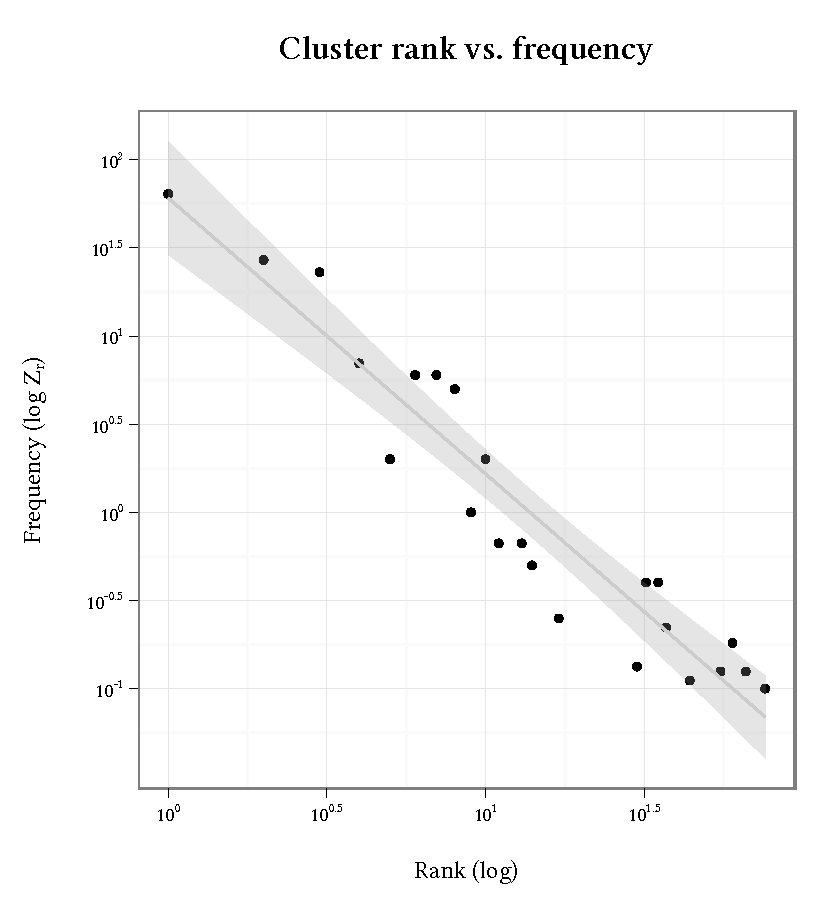
\includegraphics{cluster.pdf}
\caption{Syllable contact clusters exhibit a log-log linear relationship between frequency and rank that is consistent with Zipf's Law.}
\label{clus}
\end{figure}

Sparse distributions characterize the frequencies of many linguistic objects, from syntactic rules \citep{Yang2009} to word \citep{Teahan1998,Baroni2009} and phoneme \citep{Belevitch1956,Daland2011a} $n$-grams, but are also found in non-linguistic symbol systems \citep{Mandelbrot1954,Miller1957,Chomsky1958,Sproat2010} and randomly generated texts \citep{Miller1957,Li1992}. The importance of sparsity in this context is that it entails a long right tail, making it difficult to determine on statistical grounds alone which unobserved events are impossible and which are accidental gaps.

\subsection{The Good-Turing estimate}

One way to quantify the possibility of accidental gaps is proposed by \citet{Good1953}, who proposes an estimate of $\hat{p}_0$, the probability of all unseen events. This probability is simply $n_1$, the number of events which occur just once, divided by the number of observations.

\begin{unlabeledexample}
$\displaystyle \hat{p}_0 = \frac{n_1}{\displaystyle\sum N}$
\end{unlabeledexample}

\noindent In CELEX, $65$ clusters occur only once, and there are 873 cluster tokens, so $\hat{p}_0 = 0.074$. This indicates that were it possible to generate a new corpus of syllable contact clusters with the same statistical properties as the English data, approximately 7\% of the tokens would be clusters not found in the previous sample.

\subsection{Sampling simulation}

One possible way to generate a new corpus is by simulation, in which new clusters are generated using the following procedure, which combines the derived constraint baseline with the model proposed by \citet{Pierrehumbert1994}.

\begin{example}[Simulation procedure]
\begin{tabular}{l l}
a. & Sample a medial coda according to the observed probabilities  \\
b. & Sample a medial onset according to the observed probabilities \\
c. & Apply all matching \emph{SPE} rules to the resulting clusters \\
\end{tabular}
\end{example}

While this procedure can be repeated indefinitely, it is worthwhile to consider the results of a single characteristic ``lexicon'' produced in this fashion. The slope of the log-rank/log-frequency relationship for the simulated data ($\alpha = -0.524$) is also close to the observed slope for the CELEX data ($\alpha = -0.588$). And, as shown in Figure \ref{sim}, the two distributions are nearly indistinguishable.

\begin{figure}
\centering
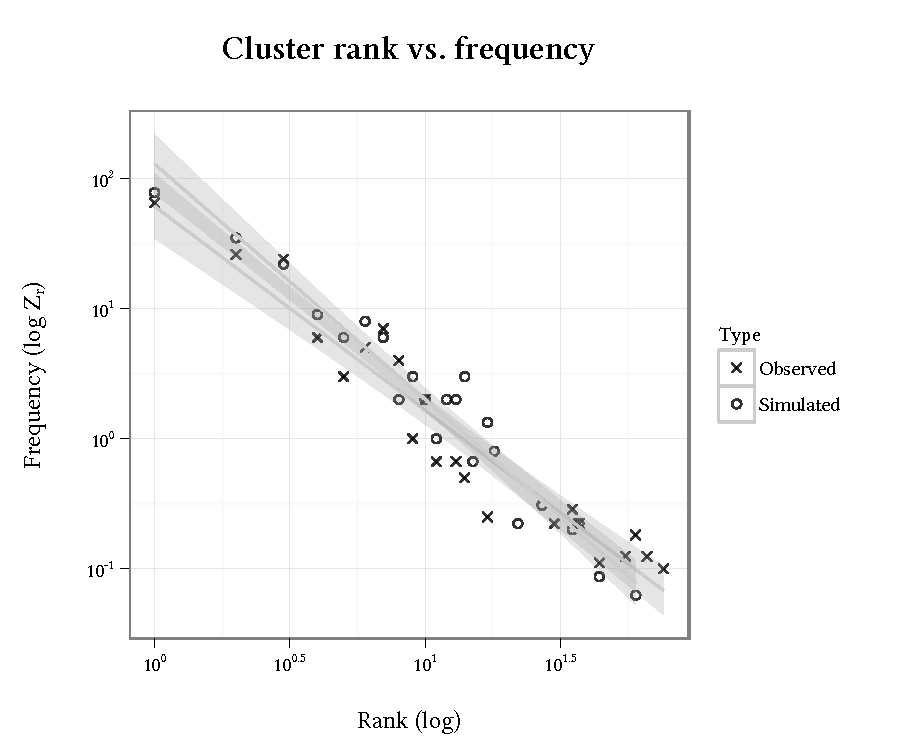
\includegraphics{sim.pdf}
\caption{The observed cluster frequencies are closely matched by a simulated cluster inventory generated by random sampling.}
\label{sim}
\end{figure}

This result should not be construed as an endorsement of the \citet{Pierrehumbert1994} model. Rather, it shows that even if the only constraints on syllable contact clusters are that they must consist of valid medial codas and onsets which further conform to the three derived constraints, there still will be many gaps in the cluster inventory, gaps which are quite arbitrary from the perspective of the phonology and phonological representations in general.

%as in \emph{a}[b.s]\emph{inth} and \emph{a}[s.b]\emph{estos} CELEX also contains \emph{jo}[d.p]\emph{urs}, \emph{pi}[ntʃ.b]\emph{eck}, \emph{sa}[k.b]\emph{ut}, and \emph{ja}[k.d]\emph{aw}. 
%There is no duplication between constraints on sequence structure and surface forms if both are derived from the application of the phonological rule (\citealt[][401f.]{Stanley1967}, \citealt[][382]{SPE}). 
%\citet{Wright1975} taught several nonce words to a group of adolescents, and asked them to repeat the words to each other in a game of ``Telephone''. In these nonse words, nasals do not agree in \textsc{Place} with the following obstruent in these nonsense words, and \citeauthor{Wright1975} observes that after a few rounds of the game, the nonce words had been adapted to conform to \textsc{Coda Nasal Place Assimilation}.
%\begin{example}[Artificial language adaptations (\citealt{Wright1975}:394, his transcriptions)]
%\begin{tabular}{l l l l}
%a. & [ɡownp] & \textgreater{} & [ɡump]  \\
%b. & [ǰumɡ]  & \textgreater{} & [ǰúŋɡuə] \\
%c. & [ðʌŋd]  & \textgreater{} & [tɔŋɡ]  \\
%\end{tabular}
%\end{example}
%\noindent If this game is akin to the process of loanword adaptation, it is possible that various extragrammatical pressures are at play \citep[e.g.,][]{Halle1998b,Dupoux1999,Ussishkin2003,Peperkamp2008}. Yet, the independent evidence for a phonological process of nasal place assimilation provides the most parsiminious account of the adaptations seen in \citeauthor{Wright1975}'s study. 
%\citet{Hay2004a} demonstrates that [n.p, mθ] clusters, which are not found in English, are in fact rated better than many attested clusters.
%The same is true of the prefix \emph{com-}/\emph{con-}, as shown by the presence of assimilation in \emph{có}[ŋ.ɡ]\emph{ress} but not in \emph{co}[n.g]\emph{réssional}. 
%(e.g., \citealt{Bakovic2005b}, \citealt{Fruehwald2011}), 

%\ex \textsc{Coda Nasal Place Assimilation} feeds \textsc{Degemination} \citep[][116]{Borowsky1986}: \\
%\begin{tabular}{l l l l}
%a. & mature    & i[m]ature    & (cf. \emph{i}[m.b]\emph{alance})   \\
%b. & numerable & i[n]umerable & (cf. \emph{i}[n.d]\emph{ependent}) \\
%\end{tabular}
%\xe
%(\citealp{Halle1985a}:105, 
%; presumably, this generalization is limited to this one place feature because  \citeauthor{Pierrehumbert1994} also adopts the assumption that the velar nasal is derived from /n/. 
%Finally, \citet{Buchwald2005} considers [j] onglides in the speech of VBR, an aphasic patient who has difficulties producing complex onsets. 
%
%\begin{example}[VBR's complex onsets (\citealp{Buchwald2005}:79--80, his transcriptions)] \label{VBR}
%\begin{tabular}{l l l}
%a. & kəræb  & `crab'  \\
%   & bəlid  & `bleed' \\
%b. & kəwin  & `queen' \\
%   & kəwoʊt & `quote' \\
%c. & kut    & `cute'  \\
%   & musɪk  & `music  \\ 
%\end{tabular}
%\end{example}
%
%\noindent VBR breaks up complex onsets with epenthesis, including those that consist of a consonant and a back onglide cluster (\ref{VBR}b). However, no epenthesis occurs between a consonant and a front onglide; rather, the glide is absent (\ref{VBR}c). The failure of the front onglide to pattern with other consonant clusters suggests once again that the glide is part of the nucleus. 
%One potential problem with this account is noted by \citet{Kaye1996}, who obseres while [juː] may follow any single tautosyllabic consonant, it never follows branching onsets unless they consist of [s] and a single consonant.This is the only sign that [juː] shows an affiliation for the onset. 
%In fact, [t.ʃ, d.ʒ] clusters are not found in simplex English words, despite the fact that that affricates occur as medial onsets in clusters (e.g., \emph{tru}[n.tʃ]\emph{eon}, \emph{so}[l.dʒ]\emph{er}).
%Finally, \citet[][251]{Fromkin1973} also presents evidence that post-vocalic \emph{r} may behave as if nuclear in speech errors. 
%\citep[e.g.,][142]{Mester1988}.
%\footnote{English glides are transcribed here as full segments, not as ``subsegments'', as this distinction does not appear to be meaningful for English, or a part of a contrast in any known language \citep{Rubach2002}.}
% Note that [tʃ] has not been included since it so rarely occurs in clusters.
%\subsubsection{Summary}
%
%The above results are summarized in Table \ref{constraints}.
%
%\begin{table}
%\centering
%\begin{tabular}{l r r r r r}
%\toprule
%                                       & \multicolumn{2}{c}{attested} & \multicolumn{2}{c}{unattested} & \multirow{2}{*}{$p$-value} \\
%                                       & conforming & violating & conforming & violating \\
%\midrule
%\textsc{O.V.A.} (\ref{ovar})        &  80 &   6 & 370 & 264 & 1.1\e{-11} \\
%\textsc{C.N.P.A} (\ref{CNPA})       &  41 &  25 &  12 &  42 & 1.7\e{-05} \\ 
%\textsc{Degemination} (\ref{degem}) & 161 & 632 &   0 &  87 & 1.4\e{-08} \\
%\midrule
%\textsc{*Dorsal-Labial} ()          &  68 &   4 & 246 &  40 & 0.069 \\
%\textsc{*C.C.O.} ()                 &  48 &  38 & 312 & 322 & 0.301 \\
%\textsc{*A,BA} ()                   & 161 &   0 & 708 &  11 & 0.231 \\
%\bottomrule
%\end{tabular}
%\caption{Counts and Fisher exact test $p$-values for the constraints discussed above.}
%\label{constraints}
%\end{table}
%Whereas 18.8.\% of the ``possible'' clusters are attested, 28.8\% of those which conform to these three constraints are found. 
%Binary classification contingency table: \\
%\begin{tabular}{c | l l} \toprule
%                             & \multicolumn{2}{c}{prediction} \\
%\midrule
%\multirow{2}{*}{observation} & true positive ($tp$)  & false positive ($fp$) \\
%                             & false negative ($fn$) & true negative ($tn$) \\
%\end{tabular}
%\begin{tabular}{|l l|}
%\toprule
%true positive ($tp$)  & false positive ($fp$) \\
%false negative ($fn$) & true negative ($tn$) \\
%\bottomrule
%\end{tabular}
%\begin{figure}
%\centering
%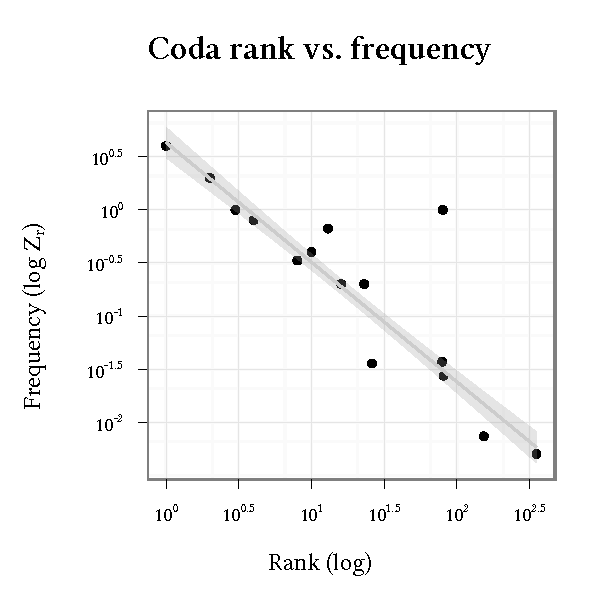
\includegraphics{coda.pdf} 
%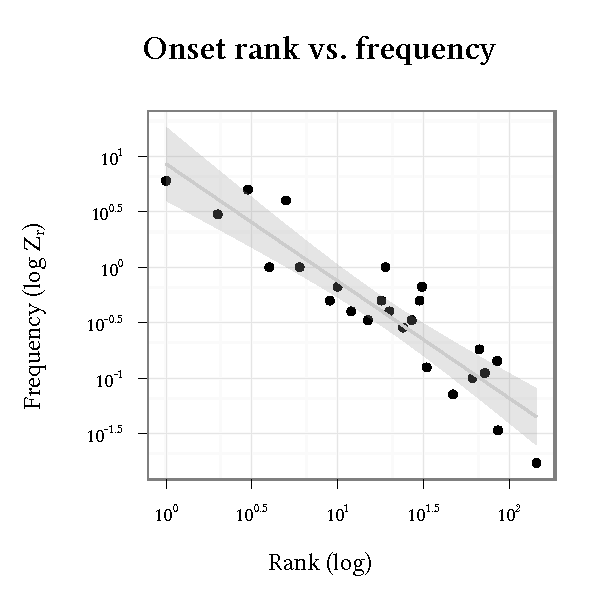
\includegraphics{onset.pdf}
%\caption{Medial coda and medial onset lexical frequency exhibit the Zipfian log-log-linear relationship between rank and frequency.}
%\label{codaonset}
%\end{figure}
%Sparsity alone is not the only reason for cluster underrepresentation which is external to the phonology. For instance, a cluster could be underrepresented due to language change. \citet{Iverson2005} discuss a case of this type: In English, long vowels before word-final [ʃ] in English are generally rare (though note ``affective'' \emph{swoosh}, \emph{sheesh}, etc.). This is ultimately due to the fact that native [ʃ] is descended from Old English [sk], and long vowels are not fonud not occur before complex codas. \citeauthor{Iverson2005} conclude that this gap is accidental because it does not inhibit borrowing and coinage. 
%On the other hand, patterns created by sound change are not guaranteed to persist over time. One example of non-persistence is discussed by \citet{Iverson2005}. Around 1100 CE, Old English \emph{sk} became [ʃ]. This sound change introduced no alternations. Since long vowels were not found before tautosyllabic syllable clusters at this time, there were no \emph{Vːsk\#} words when the change was actuated, and \emph{Vːsh\#} continues to be rare in Modern English. What \citeauthor{Iverson2005} observe, however, is that there is nothing apparently peripheral about words like \emph{leash} or \emph{whoosh}, and loanwords and coinages have readily filled the gap.
%\citet[][140]{Frisch2004} suggest that the strong tendency for the first and second consonants of the Arabic root to be non-identical is the ``a diachronic result of a processing constraint that disfavors repetition.'' Unfortunately, there is no evidence that this pattern is diachronic other than in the sense that it appears to be inherited from the proto-language: there is simply no Proto-Semitic verb roots with identical first and second consonants \citep[][178]{Greenberg1950}. In other Semitic languages, the inherited patern has experienced considerable erosion. 
%\begin{example}[Tigrinya roots with identical first and second consonants \citep{Buckley1990a}]
%\begin{tabular}{l l l l}
%a. & lʌlʌw     & `scorch'                   & (\textless{} Ge'ez \emph{lʌwlʌw} `inflame')     \\
%   & mʌmʌy     & `winnow'                   & (\textless{} Ge'ez \emph{mʌymʌy} `distinguish') \\
%   & mʌmʌt     & `pick out loot'            \\
%b. & s’ʌs’ʌw   & `finish off a drink'       & (cf. \emph{s’ʌws’ʌw} `gulp down')           \\
%   & t’ʌt’ʌf   & `prune tree'               & (cf. \emph{t’ʌft’ʌf} `smear wall with mud') \\
%c. & kʷakʷkʷʌr & `waste away, be emaciated' & (cf. \emph{kʷarkʷʌr} `interrogate')         \\
%   & kakʷkʷɨʕ  & `clean wax from ears'      & (cf. \emph{kaʕkʷɨʕ} `start to form pods')   \\
%\end{tabular}
%\end{example}
%Similar exceptions are found in 
%Amharic (\citealp[][?]{Broselow1984}, \citealp[][?]{McCarthy1985}) and 
%Hebrew \citep[][29]{Bat-El2005}.
%And onsets followed by [w] pattern with other complex onsets in undergoing epenthesis in the patholical speech of VBR, discussed immediately above.
%Before the dawn of generative phonology, many linguists concerned themselves with documenting co-occurrence in various languages. \citet[][28]{Vogt1954} declares that a ``phonemic description of a language \ldots should also comprise a description of the phoneme combinations that occur or may be expected to occur in the language''. Studies in this tradition include the discussions of consononantal co-occurrence in Arabic and Javanese by \citet{Greenberg1950} and \citet{Uhlenbeck1950}, respectively. \citeauthor{Uhlenbeck1950}, for instance, puts forth co-occurrence dispreferences, rather than exceptionless generalizations of the sort given by \citet{Greenberg1950}.
%\citet{McCarthy1988}
%Years later, \citet{Mester1988} revisits \citeauthor{Uhlenbeck1950}'s study and proposes a statistical technique, based on the chi-square test, to distinguish between accidental and structural lexical dispreferences in the Javanese lexicon. 
%\citeauthor{Mester1988}'s technique has been adopted by many subsequent studies (e.g., \citealt{Padgett1992,Padgett1995} on Russian; \citealt{Pierrehumbert1993}, \citealt{Frisch1996}, and \citealt{Frisch2004} on Arabic; \citealt{Berkley1994b,Berkley1994a,Berkley2000} on English). The null hypothesis $H_0$ is that some sequence occurs at no different a rate than the researcher expects, and the alternative hypothesis $H_1$ is that it is underrepresented. Given an observed frequency $O$ and also a frequency $E$ expected under the null hypothesis, the test is as follows.
%\begin{example}[null hypothesis testing]
%$\displaystyle \textrm{Reject } H_0 \textrm{ iff } \frac{(O E) ^ 2}{E} > χ^2$
%\end{example}
%\footnote{This is the one-tailed version of the test.}
%In this study, I use the \citet{Fisher1934} exact test, which is isomorphic to this chi-square test. Compared to the chi-square test, the Fisher exact test $p$-value is somewhat more difficult to compute, but both are automated by modern statistical packages and can be computed rapidly. The major advantage of the Fisher test over the chi-square test is that it is appropriate for small samples or rare events, whereas the chi-square test depends on an approximation which is only exact in the limit (i.e., with a hypothetically infinite sample), and therefore is not appropriate for small samples.
%On the other end of the spectrum, the Monte Carlo statistical procedure developed by \citet{Kessler2001} and applied to co-occurrence statistics by \citet{Martin2007,Martin2011} and \citet{Brown2010} does not scale to large samples. The Monte Carlo procedure is isomorphic to the one-tailed Fisher Exact test, and involves comparing observed co-occurrence counts to those produced by randomly generated samples.  This requires the researcher to generate random permutations, something which is particularly difficult for large samples, as I will explain; disinterested readers may wish to skip the following paragraph.
%Any permutation of a sequence $L$ can be represented as a sequence $S$ of the same length, where the value of $S_i$ corresponds to the permuted position of $L_i$. Generating random permutations requires an unbiased method to generate all $N!$ of these lists with equal probability. Unfortunately, this is near impossible for $N$s of moderate size with current computational resources. Any pseudo-random number generator can be characterized by its ``period'', the number of pseduo-random numbers it can emit before repeating itself; this is also the upper limit for the number of random permutations that can be generated. The pseudo-random number generator used by both \citeauthor{Martin2011} and \citeauthor{Brown2010} has a period of approximately $2^{48}$, a number which turns out to be smaller than $17!$. For the large samples, sometimes in the thousands, used by these researchers, virtually all the possible permutations can never be generated by this method. As a consequence, the shuffling procedure is far from random and introducing the possibility that the statistical test is biased in unpredictable ways.
%As an example of the Fisher exact test as it is applied here, consider some of the Javanese co-occurrence facts considered by \citet{Mester1988}. \citeauthor{Mester1988} is at pains to show that there is a gradient dispreference for first and second root consonants which share the same major place. However, perfectly identical first and second consonants are exempt. Since 
% APPLY THIS TO JAVANESE
%\begin{example}[Javanese root co-occurrence] %(\citealp[][264]{Uhlenbeck1950}, \citealp[][139]{Mester1988})]
%\begin{tabular}{l r r r r}
%\toprule
%           & attested & unattested & saturation & $p$-value \\
%\midrule
%conforming & 134      & 12         & 0.918      & \multirow{2}{*}{6.095\e{-06}} \\
%violating  & 21       & 15         & 0.583 \\
%\bottomrule
%\end{tabular}
%\end{example}
%\noindent It is evident that roots with identical labial stops are far more common than those in which the roots disagree in voicing. 
%This data is input to a chi-square test, which reports that this highly skewed distribution is unlikely to be due to chance 
%That this is highly unlikely to be due to chance is apparent both from the chi-square ($\chi^2 = 25.572$, two-tailed $p = 4.3$\e{-07}) and Fisher exaact tests ($p =  6.095$\e{-06}). 
%\citep[e.g.,]{Brown2010} have argued for phonotactic constraints giving rise to overrepresentation, so I admit this possibility here and use two-tailed tests throughout. 
%\footnote{For example, \citet{Martin2007} applies this technique to a list of 4,758 noun-noun compounds. The number of permutations of a list of this length can be estimated using Stirling's approximation.
%\ex $ \lim_{n \rightarrow \infty} n! = e ^ {n \ln{n} - n} = 2 ^ {\log_2{e} (n \ln{n} - n)} $ \xe
%$4,758!$ is approximately $2 ^ {51260}$. The author is unaware of any system that provides 51,260 bits of entropy; and some popular programming languages, such as ANSI C, provide as few as 15 bits.}
%With this database of English syllable contact clusters it is now possible to evaluate constraints on sequences of underlying phonemes. 
%I now consider constraints on sequences of URs as predictors of attested and unattested contact clusters. 
%Two-tailed statistical tests are used throughout.
%\citet[56]{Coppock2008} observes that there is every reason to believe that the ditransitive is productive in the sense that it can be applied to new words; consider recent conversion \emph{text} (e.g., \emph{text me your number}). 
%\footnote{\citet[][589f.]{Lowenstamm1981} observes a strikingly similar issue with the onset maximization principle in French, and proposes a similar solution.}
%Despite this, six of the eight words that \citet[172]{Pierrehumbert1994} labels ``reasonably familiar'' (and thus included) are included in this study (\emph{velcro} and \emph{eclampsia} are not found in CELEX), and none of the five examples of words which are not ``reasonably familiar''.
%between irregular verbs and their base forms \citep{Allen2002,Stockall2006}
%\begin{quote}
%These regularities, although not the products of alternations, are described and defined by elements of phonological theories: segments\ldots{}and distinctive features. \citep[13]{Berkley2000}
%\end{quote}
%One of the first study of this type was an analysis of co-occurrence restrictions on consonants in Javanese roots by \citet{Mester1988}, recently revisited by \citet{Graff2011}. Another Austronesian language studied in this fashion is Muna \citep{Coetzee2008a,Anttila2008}. This technique has been applied to consonants in Semitic, especially Arabic \citep{McCarthy1988,McCarthy1994,Pierrehumbert1993,Frisch1996,Frisch2004,Coetzee2008a}) but also in Tigrinya \citep{Buckley1997}, Hebrew \citep{Berent2003}, and Amharic \citep{Colavin2010}, and to various co-occurrence restrictions in English \citep{Berkley1994b,Berkley1994a,Pierrehumbert1994,Coetzee2008b}, Russian \citep{Padgett1992}, Dutch \citep{Graff2011}, Navajo \citep{Martin2007,Martin2011} and Gitksan \citep{Brown2010}.
%\begin{quote}
%\ldots{}the fact that some [clusters--KG] are not found must be due to accidental gaps in the inventory of signs, and cannot be explained by structural laws of the language. \citep[][16]{Fischer-Jorgensen1952}
% 
%Although my material is drawn from a fairly extensive corpus---all accessible dictionaries and vocabularies, printed texts of tens of thousands of pages as well as ordinary speech---there is every reason to believe, as experience has shown, that additional material would yield new clusters. The material will never be complete. It will always contain accidental gaps \ldots partly because some clusters by pure chance do not occur in the vocabulary. \citep[][30]{Vogt1954}
%\end{quote}
%\begin{quote}
%Of course, to obtain the desired results, we must guarantee that each sequence structure rule reflects a general systematic fact about the language, and not a fact which is due merely to the existence of accidental gaps in the lexicon. \citep[][401, fn.~8]{Stanley1967}
%
%In describing and explaining the phonotactic patterns in any language, phonologists recognize a distinction between accidental and systematic gaps in the lexicon\ldots{}A gap is taken to be systematic if it belongs to a natural class of examples according to the current theory of the investigator. Otherwise it is viewed as accidental.\citep[][180]{Frisch2004}
%\end{quote}
%\footnote{At this juncture it is necessary to clarify a persistent confusion in the literature: commitment to a negative heuristic like Stampean occultation or Richness of the Base \citep{OT} does not entail an adoption of a particular algorithm, lke Lexicon Optimization, which produces a grammar consistent with these heuristics. For instance, Lexicon Optimization is incapable of converging on a grammar of English in which [k] derives from an underlying dorsal click \citep[73]{PE}. Yet, such a grammar is entirely consistent with Richness of the Base.}
